\documentclass{beamer}

\usetheme{metropolis}

\metroset{
  progressbar=frametitle,   % thin progress bar under each title
  block=fill,
  numbering=fraction        % "3/12" instead of just "3"
}
\usepackage{graphicx}
\usepackage{booktabs}
\usepackage{amsmath}
\usepackage{tikz}
\usetikzlibrary{arrows.meta, positioning}
\usepackage{adjustbox}

% tables in tables/ are generated by Section 18 of football-wk4-nestedtune.R (kable, booktabs)
% shrunk only if wider than the column, never enlarged
\newcommand{\rtable}[1]{\adjustbox{max width=\linewidth}{\input{tables/#1.tex}}}
\newcommand{\todo}[1]{\textcolor{gray}{[#1]}}

\title{Case Studies: Sports Analytics}
\subtitle{UEFA Euro -- Poisson, Skellam W/D/L and the draw problem}
\author{Nicholas, Sriram, Rohit, Silas}
\date{}

\begin{document}

\maketitle

% ------------------------------------------------------------------
\begin{frame}
  \frametitle{Research Question}

  \begin{itemize}
    \item Predict \textbf{win / draw / loss} for UEFA Euro 2028 matches from
          team covariates (GDP, market value, FIFA rank, UEFA points,
          Champions League players, group stage)
    \item Which model class and which tuning metric give the best
          \textbf{honest out-of-sample} W/D/L performance?
    \item In particular: can we predict \textbf{draws} at all?
  \end{itemize}

  \vspace{0.5em}
  \textbf{This week:} Poisson elastic net in depth
  \begin{itemize}
    \item goals $\rightarrow$ Skellam $\rightarrow$ W/D/L $\rightarrow$ draw threshold
    \item evaluated with nested leave-one-Euro-out cross-validation
  \end{itemize}

\end{frame}

% ------------------------------------------------------------------
\begin{frame}
  \frametitle{Assumptions}

  \begin{itemize}
    \item \textbf{Goal is 2028, not 2024}: past Euros stand in for the future one
    \begin{itemize}
      \item assumes dependence over time between Euros is negligible
      \item e.g.\ squad market values have grown a lot since 2004; comparing the two
            teams of a match limits this, remaining drift is assumed negligible
    \end{itemize}

    \item \textbf{Respect \texttt{match\_id} in the split}
    \begin{itemize}
      \item each match is two mirror-image rows (team vs opponent, covariates $x$ and $-x$)
      \item splitting them across train/test would leak the result
    \end{itemize}

    \item \textbf{Respect tournament / year in the split}
    \begin{itemize}
      \item a team's covariates (e.g.\ its 2024 market value) repeat in all its
            matches of that Euro
      \item random row splits would let the model see the test tournament
            $\rightarrow$ optimistic scores
    \end{itemize}
  \end{itemize}

\end{frame}

% ------------------------------------------------------------------
\begin{frame}
  \frametitle{Model Class Choices}

  \centering
  \resizebox{\linewidth}{!}{%
  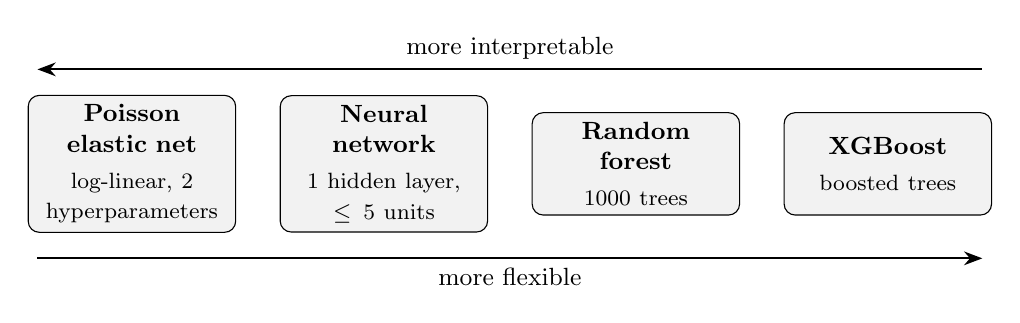
\begin{tikzpicture}[
      model/.style={draw, rounded corners, fill=gray!10, text width=2.4cm,
                    align=center, minimum height=1.3cm, font=\small},
      >=Stealth]
    \node[model] (pois) at (0,0)    {\textbf{Poisson elastic net}\\[2pt]\footnotesize log-linear, 2 hyperparameters};
    \node[model] (nn)   at (3.2,0)  {\textbf{Neural network}\\[2pt]\footnotesize 1 hidden layer, $\le 5$ units};
    \node[model] (rf)   at (6.4,0)  {\textbf{Random forest}\\[2pt]\footnotesize 1000 trees};
    \node[model] (xg)   at (9.6,0)  {\textbf{XGBoost}\\[2pt]\footnotesize boosted trees};

    \draw[->, thick] (-1.2,-1.2) -- node[below, font=\small] {more flexible} (10.8,-1.2);
    \draw[<-, thick] (-1.2, 1.2) -- node[above, font=\small] {more interpretable} (10.8, 1.2);
  \end{tikzpicture}}

  \vspace{0.3em}
  \small
  \begin{itemize}
    \item All classes predict \textbf{goals per team}, then share the same
          Skellam W/D/L step (NN also tried direct classification)
    \item Same nested split structure for every class $\rightarrow$ comparable scores
    \item This week's deep dive: the Poisson elastic net
  \end{itemize}

\end{frame}

% ------------------------------------------------------------------
\begin{frame}
  \frametitle{Choosing Evaluation Metrics}

  \centering
  \resizebox{\linewidth}{!}{%
  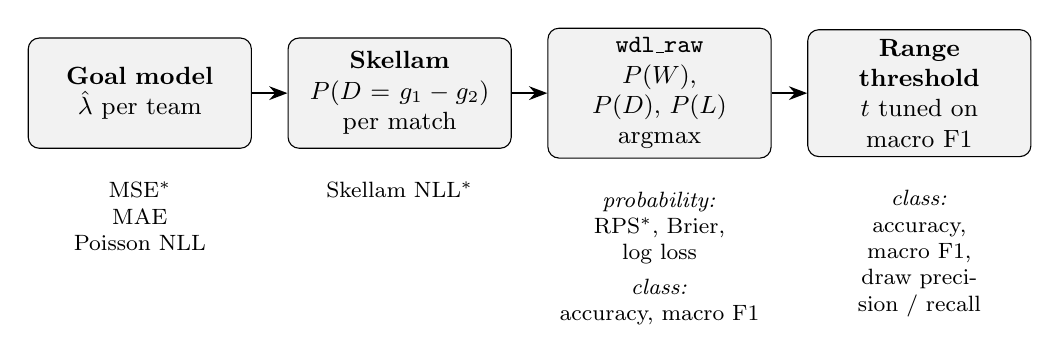
\begin{tikzpicture}[
      stage/.style={draw, rounded corners, fill=gray!10, text width=2.6cm,
                    align=center, minimum height=1.4cm, font=\small},
      met/.style={text width=2.6cm, align=center, font=\footnotesize},
      >=Stealth]
    \node[stage] (g) at (0,0)    {\textbf{Goal model}\\$\hat\lambda$ per team};
    \node[stage] (s) at (3.3,0)  {\textbf{Skellam}\\$P(D = g_1 - g_2)$\\per match};
    \node[stage] (w) at (6.6,0)  {\textbf{\texttt{wdl\_raw}}\\$P(W)$, $P(D)$, $P(L)$\\argmax};
    \node[stage] (t) at (9.9,0)  {\textbf{Range threshold}\\$t$ tuned on\\macro F1};
    \draw[->, thick] (g) -- (s);
    \draw[->, thick] (s) -- (w);
    \draw[->, thick] (w) -- (t);

    \node[met, below=0.3cm of g] {MSE$^\ast$\\MAE\\Poisson NLL};
    \node[met, below=0.3cm of s] {Skellam NLL$^\ast$};
    \node[met, below=0.3cm of w] {\textit{probability:}\\RPS$^\ast$, Brier, log loss\\[3pt]\textit{class:}\\accuracy, macro F1};
    \node[met, below=0.3cm of t] {\textit{class:}\\accuracy, macro F1,\\draw precision / recall};
  \end{tikzpicture}}

  \vspace{0.2em}
  \footnotesize
  \begin{itemize}
    \item All considered: macro F1, RPS, Poisson NLL, MSE, MAE, Skellam NLL
    \item $^\ast$ used as the hyperparameter \textbf{selection} metric (one experiment each)
    \item Probability metrics don't depend on $t$; class metrics are reported
          for argmax (\texttt{wdl\_raw}) and for the tuned threshold
  \end{itemize}

\end{frame}

% ------------------------------------------------------------------
\begin{frame}
  \frametitle{Draws Are Under-Predicted}

  \begin{columns}[T]
    \begin{column}{0.44\textwidth}
      \footnotesize
      \textbf{Argmax W/D/L}, nested outer predictions (selected on RPS)

      \vspace{0.4em}
      \centering
      \scriptsize
      \setlength{\tabcolsep}{4pt}
      \adjustbox{max width=\linewidth}{%
      \begin{tabular}{lrrr}
        \toprule
        & \multicolumn{3}{c}{actual} \\
        \cmidrule(lr){2-4}
        predicted & win & draw & loss \\
        \midrule
        win  & 64 & 34 & 30 \\
        draw &  0 &  0 &  0 \\
        loss & 23 & 38 & 57 \\
        \bottomrule
      \end{tabular}}

      \vspace{0.6em}
      \raggedright
      \begin{itemize}
        \footnotesize
        \item 72 of 246 matches are draws (29\%)
        \item argmax calls \textbf{0} draws
        \item max predicted $P(D)$ = 0.29, mean 0.26
        \item historical-frequency baseline: also 0 draws
      \end{itemize}
    \end{column}

    \begin{column}{0.54\textwidth}
      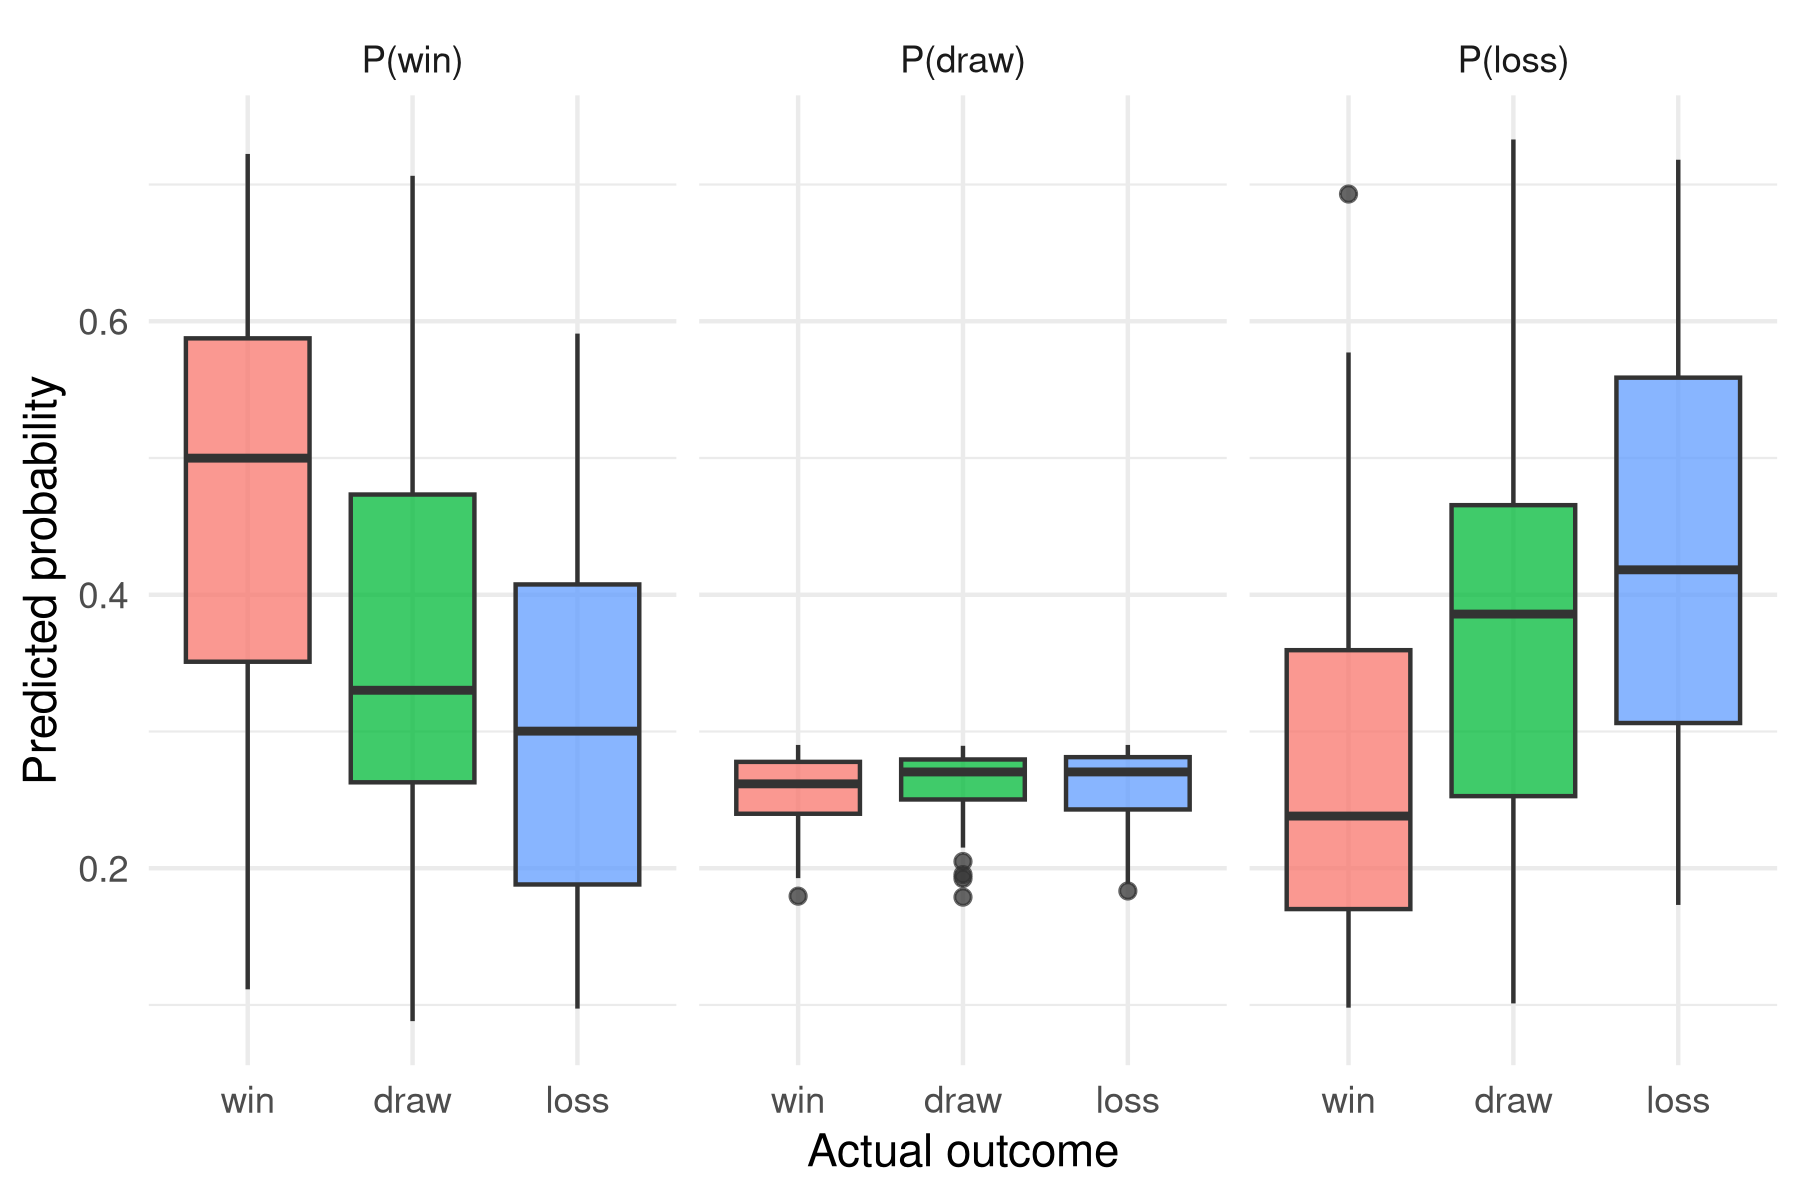
\includegraphics[width=\textwidth]{wdl_pois_rps_box.png}
    \end{column}
  \end{columns}

\end{frame}

% ------------------------------------------------------------------
\begin{frame}
  \frametitle{Approach to Fixing Draw Prediction}

  \small
  \textbf{Range idea:} a match is a toss-up when the three probabilities are close
  \[
    \text{draw if }\; \max(P_W, P_D, P_L) - \min(P_W, P_D, P_L) < t,
    \;\text{ else argmax}
  \]

  \vspace{-0.6em}
  \begin{columns}[T]
    \begin{column}{0.52\textwidth}
      \begin{itemize}
        \footnotesize
        \item Started with a pure, fixed threshold ($t = 0.15$)
        \item Then tuned $t$, first on \textbf{accuracy}: calling draws costs
              correct wins/losses, so accuracy barely rewards it
        \item Moved to \textbf{macro F1}: every class weighted equally,
              so getting draws right counts
        \item $t$ chosen \textbf{leave-one-Euro-out}: 0.25 for 5 of 6 years,
              0.225 for 2016; final rule for 2028: $t = 0.25$
      \end{itemize}
    \end{column}

    \begin{column}{0.44\textwidth}
      \centering
      \footnotesize
      Pooled outer predictions (selected on RPS)

      \vspace{0.3em}
      \begin{tabular}{rrrr}
        \toprule
        $t$ & draws & accuracy & macro F1 \\
        \midrule
        0     &   0 & 0.492 & 0.384 \\
        0.10  &  20 & 0.463 & 0.391 \\
        0.15  &  69 & 0.463 & 0.452 \\
        0.20  & 101 & 0.463 & 0.464 \\
        0.225 & 115 & 0.472 & 0.476 \\
        \textbf{0.25} & \textbf{121} & \textbf{0.476} & \textbf{0.480} \\
        0.275 & 129 & 0.463 & 0.468 \\
        0.30  & 145 & 0.455 & 0.457 \\
        \bottomrule
      \end{tabular}
    \end{column}
  \end{columns}

\end{frame}

% ------------------------------------------------------------------
\begin{frame}
  \frametitle{Draw Fix: Baseline vs Argmax vs Range-Adjusted}

  \footnotesize
  Nested outer predictions; historical-frequency baseline is leave-one-Euro-out

  \vspace{0.4em}
  \centering
  \rtable{model_comparison_class}

  \vspace{0.6em}
  \raggedright
  \begin{columns}[T]
    \begin{column}{0.44\textwidth}
      \centering
      \rtable{model_comparison_prob}
    \end{column}
    \begin{column}{0.52\textwidth}
      \begin{itemize}
        \item Probability metrics are identical for argmax and range-adjusted:
              only the decision rule changes
        \item Range adjustment: macro F1 0.38 $\rightarrow$ 0.48, draw recall
              0 $\rightarrow$ 0.54, small accuracy cost
      \end{itemize}
    \end{column}
  \end{columns}

\end{frame}

% ------------------------------------------------------------------
\begin{frame}
  \frametitle{Group Dynamics}

  \begin{itemize}
    \item \textbf{Communication:} \todo{fill in}
    \item \textbf{Work splitting:} \todo{fill in}
    \item \textbf{Meeting type:} \todo{fill in}
    \item \textbf{Git repo:} \todo{fill in}
  \end{itemize}

\end{frame}

% ------------------------------------------------------------------
\begin{frame}
    \frametitle{Poisson Elastic Net 1}

    \footnotesize

    \textbf{Hyperparameter Grid} $7 \times 7$ = 49 combinations

    {\scriptsize\centering
      $\text{penalty} \in \{1.00e\text{-}10,\; 4.64e\text{-}09,\; 2.15e\text{-}07,\;
      1.00e\text{-}05,\; 4.60e\text{-}04,\; 2.15e\text{-}02,\; 1.00\}$\\[2pt]
      $\times\;\; \text{mixture} \in \{0.000,\; 0.167,\; 0.333,\; 0.500,\; 0.666,\; 0.833,\; 1.000\}$\par
    }

    \textbf{Poisson Regression}
    \vspace{-.2cm}
    \begin{align*}
        \log(\mu(x)) &= \beta_0 + \beta^T x\\
        \ell(\beta|X,Y) &= \sum_{i=1}^N
        \left[
        y_i(\beta_0+\beta^Tx_i)
        - e^{\beta_0+\beta^Tx_i}
        \right]
    \end{align*}

    \vspace{-0.2cm}

    \textbf{Penalized Objective}

    \vspace{-0.1cm}

    \footnotesize
    \[
    \begin{aligned}
    \hat{\beta} = \arg\min_{\beta_0,\beta}
    \quad &-\frac{1}{N}\ell(\beta|X,Y) +\lambda\left[
    \frac{1-\alpha}{2}\sum_{j=1}^p\beta_j^2
    +\alpha\sum_{j=1}^p|\beta_j|
    \right]
    \end{aligned}
    \]

    \vspace{-0.3cm}

    \begin{itemize}
        \item \textbf{Penalty ($\lambda$):} Total amount of regularization.
        \item \textbf{Mixture ($\alpha$):} Proportion of L1 regularization
              ($\alpha=1$: pure lasso, $\alpha=0$: ridge regression)
    \end{itemize}

    \vfill

    \tiny
    \href{https://glmnet.stanford.edu/articles/glmnet.html\#poisson-regression-family-poisson}{glmnet Poisson regression documentation link}
    \quad
    \href{https://parsnip.tidymodels.org/reference/poisson_reg.html}{parsnip Poisson regression documentation link}

\end{frame}

% ------------------------------------------------------------------
\begin{frame}
  \frametitle{Nested CV}

    \begin{columns}[c]
        \begin{column}{0.5\textwidth}
            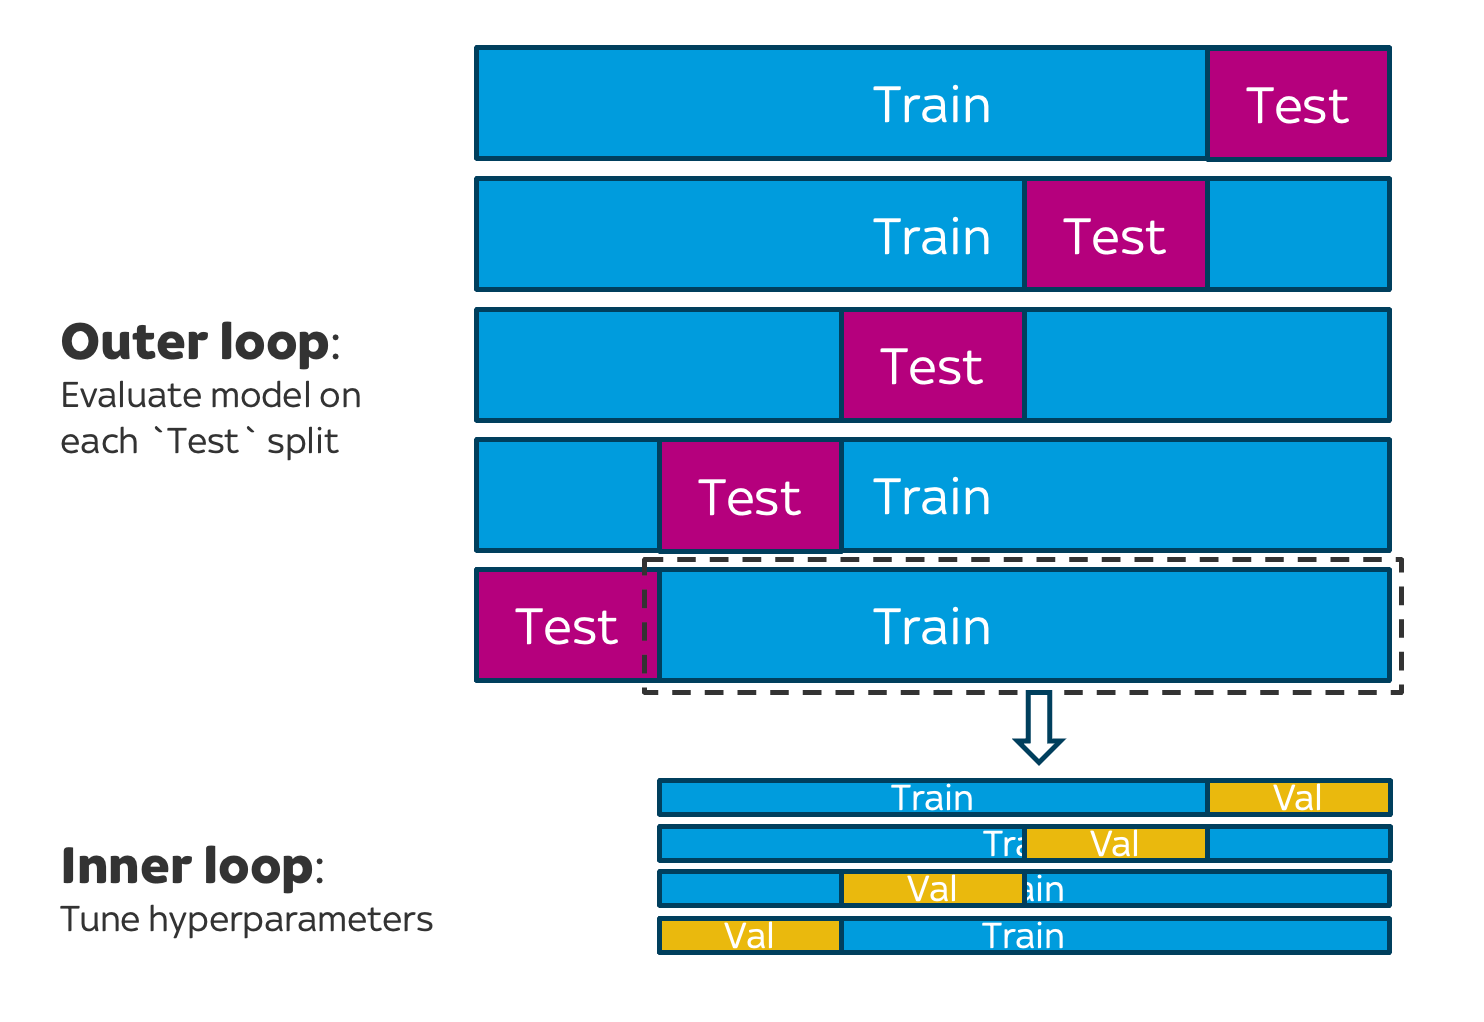
\includegraphics[width = \textwidth]{nested-cv-illustration.png}
        \end{column}
         \begin{column}{0.5\textwidth}
            {\footnotesize
            \begin{itemize}
                \item Test = 2020 (Outer 1)
                \begin{itemize}
                    \item Eval = 2024 (Inner 1.1)
                    \item Eval = 2008 (Inner 1.2)
                    \item ...
                \end{itemize}

                \item Test = 2004 (Outer 2)
                \begin{itemize}
                    \item Eval = 2020 (Inner 2.1)
                    \item Eval = 2008 (Inner 2.2)
                    \item ...
                \end{itemize}
            \end{itemize}}
        \end{column}
    \end{columns}

\textbf{Outer:} Grouped Leave One Euro Out (6 Splits)

\textbf{Inner:} Grouped Leave One Euro Out  (5 Splits x 6 Splits = 30 )


{\tiny \textbf{Image Source:} \url{https://towardsdatascience.com/two-common-pitfalls-to-avoid-when-doing-cross-validation-c68ed79c0e4e/}}


\end{frame}

% ------------------------------------------------------------------
\begin{frame}
  \frametitle{Poisson: Skellam W/D/L vs Goal-Based Selection Metrics}

  \begin{columns}[T]
    \begin{column}{0.37\textwidth}
      \footnotesize
      \textbf{Hyperparameter effects}

      \vspace{0.2em}
      \scriptsize
      \setlength{\tabcolsep}{2.5pt}
      Selected per outer fold

      \rtable{selection_comparison}

      \vspace{0.5em}
      Final (2028) models
      \rtable{pois_select_rule_hyperparams_final}

      \vspace{0.3em}
      \scriptsize
      Folds disagree, but mse and rps finals are identical;
      skellam differs only in mixture
    \end{column}

    \begin{column}{0.61\textwidth}
      \footnotesize
      \textbf{Overall performance effects}

      \vspace{0.2em}
      \scriptsize
      \setlength{\tabcolsep}{3pt}
      Nested outer, pooled (se across 6 Euros)

      \rtable{nested_eval_report}

      \vspace{0.3em}
      \scriptsize
      \texttt{\_t}: tuned range threshold, \texttt{\_raw}: argmax.
      All differences between selection metrics are well within 1 se;
      every Poisson model clearly beats the baseline
    \end{column}
  \end{columns}

\end{frame}

% ------------------------------------------------------------------
\begin{frame}
  \frametitle{Novel Covariate Finding Progress}

\end{frame}

% ------------------------------------------------------------------
\begin{frame}
  \frametitle{Poisson Coefficient Interpretation (Final Model)}

  \footnotesize
  Selected on mse and on rps (identical model): $\lambda = 0.0215$, $\alpha = 1$ (lasso)

  \vspace{0.2em}
  \centering
  {\scriptsize \rtable{pois_rps_coefs}}

  \raggedright
  \scriptsize
  \begin{itemize}
    \item $\log \lambda = \beta_0 + \sum_k \beta_k x_k$: expected goals are
          \textbf{multiplied} by $e^{\beta_k}$ per unit, $e^{\beta_k sd_x}$ per sd of $x_k$
    \item Team-minus-opponent differences: 1-sd market value advantage
          $\rightarrow \times 1.21$ expected goals ($+21\%$)
    \item UEFA points dropped by the lasso; strength covariates overlap, read them as a group
    \item Point estimates only (no standard errors from glmnet); lasso shrinks toward 0
  \end{itemize}

\end{frame}

% ------------------------------------------------------------------
\begin{frame}
  \frametitle{Poisson Final Model Validation Checks}

  \begin{columns}[T]
    \begin{column}{0.42\textwidth}
      \scriptsize
      \rtable{final_diagnostics}

      \vspace{0.3em}
      \begin{itemize}
        \item \textbf{Dispersion} $\approx 0.88$: no overdispersion
        \item \textbf{Within-match} $r = 0.05$, $p = 0.42$: Skellam's
              independence assumption holds
        \item \textbf{Log-linear form} (right): residuals scatter around 0
        \item $\Rightarrow$ draw problem is the W/D/L decision rule,
              not model misspecification
      \end{itemize}
    \end{column}

    \begin{column}{0.56\textwidth}
      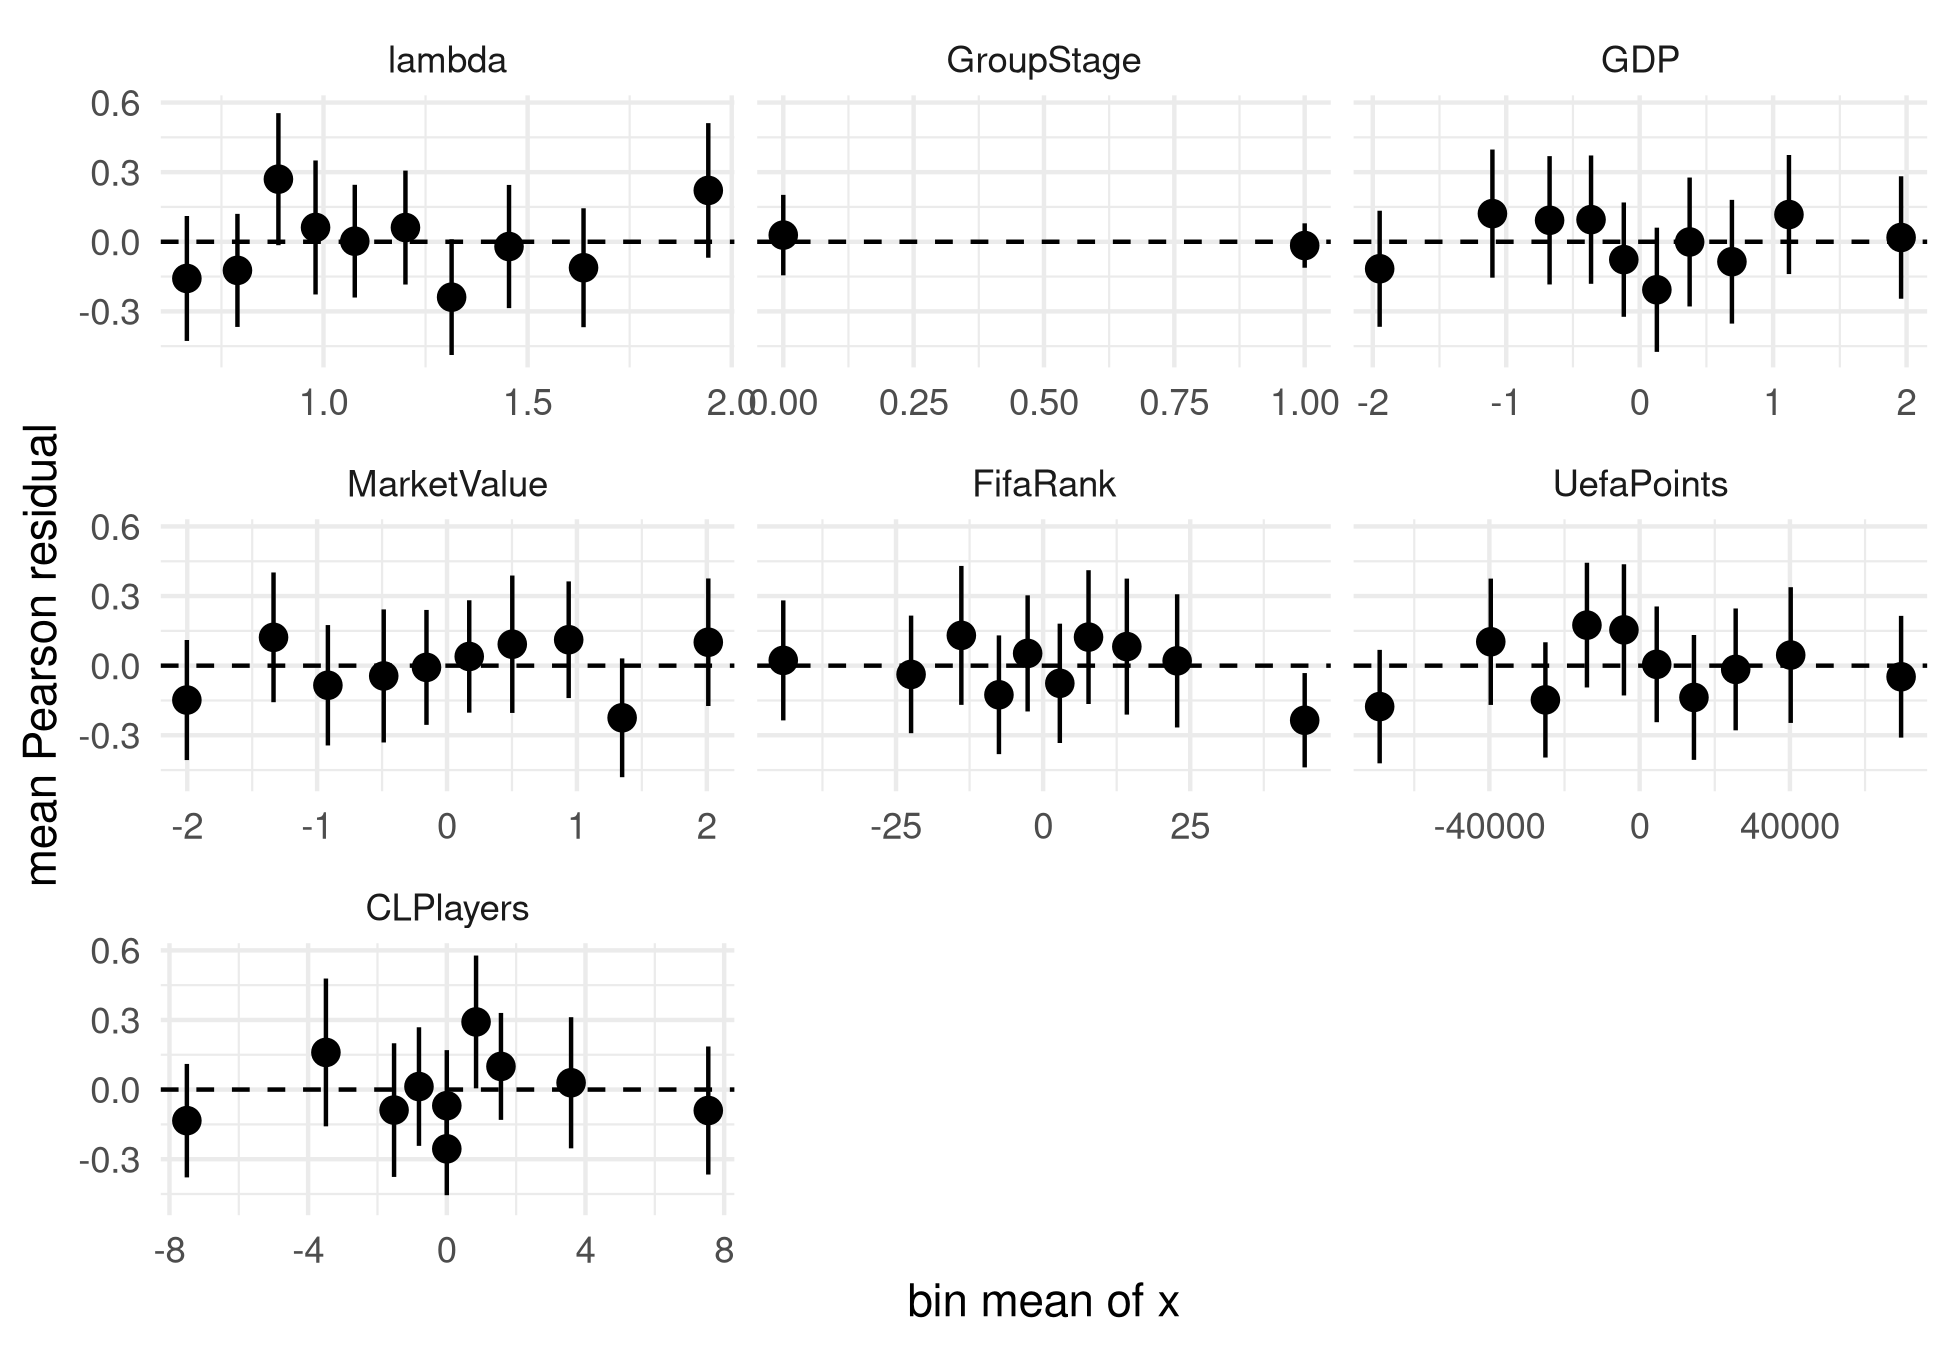
\includegraphics[width=\textwidth]{loglinear_pois_rps.png}
    \end{column}
  \end{columns}

\end{frame}

% ------------------------------------------------------------------
\begin{frame}
  \frametitle{Next Steps}

  \begin{itemize}
    \item Feature importance
    \item Potentially testing with an expanding window
          (train on past Euros only, predict the next)
    \item Standardizing data pipelines across model classes, to be sure we
          compare apples to apples
  \end{itemize}

\end{frame}

% ------------------------------------------------------------------
\appendix

\begin{frame}
  \frametitle{Backup: Final Model Selected on Skellam NLL}

  \footnotesize
  $\lambda = 0.0215$, $\alpha = 0.5$

  \vspace{0.3em}
  \rtable{pois_skel_coefs}

  \vspace{0.4em}
  Nearly identical to the mse / rps final model.

\end{frame}

\end{document}
